\documentclass{mimosis}

\usepackage{metalogo}

%%%%%%%%%%%%%%%%%%%%%%%%%%%%%%%%%%%%%%%%%%%%%%%%%%%%%%%%%%%%%%%%%%%%%%%%
% Some of my favourite personal adjustments
%%%%%%%%%%%%%%%%%%%%%%%%%%%%%%%%%%%%%%%%%%%%%%%%%%%%%%%%%%%%%%%%%%%%%%%%
%
% These are the adjustments that I consider necessary for typesetting
% a nice thesis. However, they are *not* included in the template, as
% I do not want to force you to use them.

% This ensures that I am able to typeset bold font in table while still aligning the numbers
% correctly.
\usepackage{etoolbox}

\usepackage[binary-units=true]{siunitx}
\DeclareSIUnit\px{px}

\sisetup{%
  detect-all           = true,
  detect-family        = true,
  detect-mode          = true,
  detect-shape         = true,
  detect-weight        = true,
  detect-inline-weight = math,
}

%%%%%%%%%%%%%%%%%%%%%%%%%%%%%%%%%%%%%%%%%%%%%%%%%%%%%%%%%%%%%%%%%%%%%%%%
% Hyperlinks & bookmarks
%%%%%%%%%%%%%%%%%%%%%%%%%%%%%%%%%%%%%%%%%%%%%%%%%%%%%%%%%%%%%%%%%%%%%%%%

\usepackage[
  colorlinks = true,
  citecolor  = navyblue,
  linkcolor  = navyblue,
  urlcolor   = navyblue,
  unicode,
  ]{hyperref}

\usepackage{bookmark}

%%%%%%%%%%%%%%%%%%%%%%%%%%%%%%%%%%%%%%%%%%%%%%%%%%%%%%%%%%%%%%%%%%%%%%%%
% Bibliography
%%%%%%%%%%%%%%%%%%%%%%%%%%%%%%%%%%%%%%%%%%%%%%%%%%%%%%%%%%%%%%%%%%%%%%%%
%
% I like the bibliography to be extremely plain, showing only a numeric
% identifier and citing everything in simple brackets. The first names,
% if present, will be initialized. DOIs and URLs will be preserved.

\usepackage[
  autocite     = plain,
  backend      = biber,
  doi          = true,
  url          = true,
  giveninits   = true,
  hyperref     = true,
  maxbibnames  = 99,
  maxcitenames = 99,
  sortcites    = false,
  style        = numeric,
  ]{biblatex}

\addbibresource{Thesis.bib}

%% Avoiding hyphenation
%\usepackage[none]{hyphenat}
\tolerance=1
\emergencystretch=\maxdimen
\hyphenpenalty=10000
\hbadness=10000

%%%%%%%%%%%%%%%%%%%%%%%%%%%%%%%%%%%%%%%%%%%%%%%%%%%%%%%%%%%%%%%%%%%%%%%%
% Fonts
%%%%%%%%%%%%%%%%%%%%%%%%%%%%%%%%%%%%%%%%%%%%%%%%%%%%%%%%%%%%%%%%%%%%%%%%

\ifxetexorluatex
  \setmainfont{Minion Pro}
\else
    \usepackage[sfdefault]{noto}
    %\usepackage{tgbonum}
    %\usepackage{lmodern}
    %\usepackage{dejavu}
    %\usepackage{charter}
    
    %\renewcommand{\familydefault}{\sfdefault}
    %\usepackage{bookman}
    

%%%%%%%% tgadventor %%%%
%\usepackage{tgadventor}
%    \usepackage[T1]{fontenc}
%%%%%%%%    
%%%%%%%% MONTSERRAT %%%%
%   \usepackage[defaultfam,tabular,lining]{montserrat} %% Option 'defaultfam'
    %% only if t\item \textsb{Industria arloko arauak kontsultatzeko zerbitzua}: he base font of the document is to be sans serif
%    \usepackage[T1]{fontenc}
%   \renewcommand*\oldstylenums[1]{{\fontfamily{Montserrat-TOsF}\selectfont #1}}
%%%%%%%%%%%%%%%%%%%%%%%%  
  \usepackage{cfr-lm} %%for semibold
  \usepackage{float} %%image placement
  \usepackage[oldstyle,scale=0.7]{sourcecodepro}
  \singlespacing
\fi

\renewcommand{\th}{\textsuperscript{\textup{th}}\xspace}


\newacronym{spa}{SPA}{Single Page Application}


\newglossaryentry{testing}{%
  name        = {\textbf{\emph{Testing}a}},
  description = {Software produktu batek betekizunak betetzen dituela, esperotako jarrera jarraitzen duela eta defekturik ez duela ziurtatzeko metodoa da.\\}
}



\makeindex
\makeglossaries

\setcounter{secnumdepth}{4}
\setcounter{tocdepth}{4}
%%%%%%%%%%%%%%%%%%%%%%%%%%%%%%%%%%%%%%%%%%%%%%%%%%%%%%%%%%%%%%%%%%%%%%%%
% Incipit
%%%%%%%%%%%%%%%%%%%%%%%%%%%%%%%%%%%%%%%%%%%%%%%%%%%%%%%%%%%%%%%%%%%%%%%%
\title{Bidaia: plataforma colaborativa para la organización de viajes}
\author{Josu Garralda Arrastia}

\begin{document}

\frontmatter
  
%\begin{titlepage}
%  %\vspace*{4cm}
%  \makeatletter
%  \begin{center}
%    \includegraphics[height=2cm]{Figures/orokorra/logoMGEP.png}
%    \hspace{5cm}
%    \includegraphics[height=2cm]{Figures/orokorra/logoCYC.png}
%    \vfill
 %   \begin{Huge}
 %     \@title
%    \end{Huge}\\[0.1cm]
    %
%    \vspace{0.5cm}
%    \begin{Large}
%      \@subtitle
%    \end{Large}
    %
%    \emph{}\\
%    \@author
    %
%    \vfill
    
%    \emph{Informatikako Ingeniaritza Graduko} titulua eskuratzeko lana.\\
%    \textsc{Mondragon Unibertsitatea - Goi Eskola Politeknikoa}\\
%%    \vspace{0.5cm}
%    \textsc{2021/2022 ikasturtea}
%  \end{center}
%  \makeatother
%\end{titlepage}

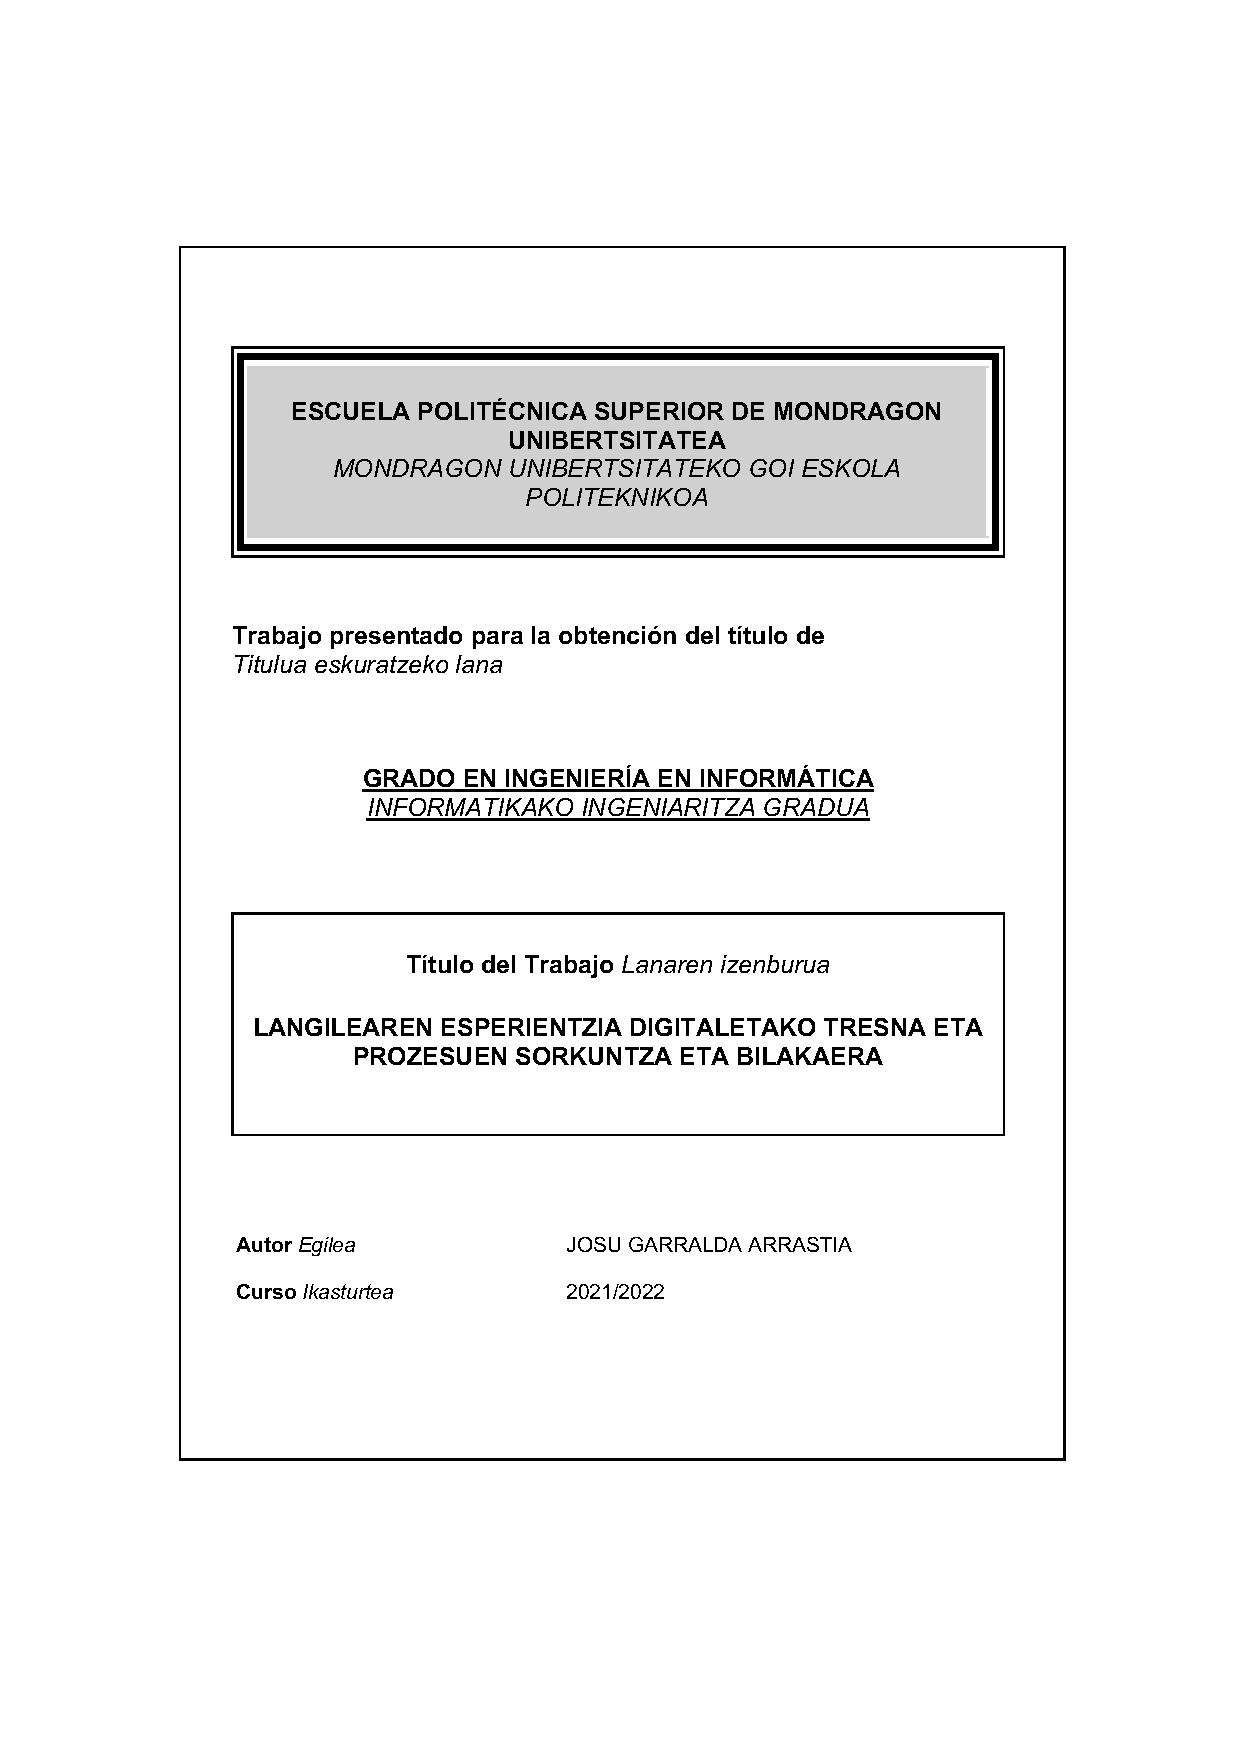
\includepdf[fitpaper=true, pages=-]{Assets/azala.pdf}

\newpage
\null
\thispagestyle{empty}
\newpage

  \chapter*{Agradecimientos}
En este documento en el que recojo el resultado del trabajo de fin de máster...

  \begin{center}
  {\Large \textsc{\textcolor{NavyBlue}{Abstract}}}
\end{center}
%
\noindent
%

\textsc{\textcolor{NavyBlue}{Keywords:}} 

\vspace{2cm}

\begin{center}
  {\Large \textsc{\textcolor{NavyBlue}{Resumen}}}
\end{center}
%
\noindent
%

\textsc{\textcolor{NavyBlue}{Palabras clave:}}
  \tableofcontents
  \listoffigures
  \listoftables

\mainmatter
  %%%%%%%%%%%%%%%%%%%%%%%%%%%%%%%%%%%%%%%%%%%%%%%%%%%%%%%%%%%%%%%%%%%%%%%%
\chapter{Introducción}
%%%%%%%%%%%%%%%%%%%%%%%%%%%%%%%%%%%%%%%%%%%%%%%%%%%%%%%%%%%%%%%%%%%%%%%%

     \parbox{1\linewidth}{En este capítulo se muestra el proceso inicial de análisis y el planteamiento del proyecto, así como los objetivos propuestos y el enfoque y método que se seguirá para poder cumplir con la planificación.}

%%%%%%%%%%%%%%%%%%%%%%%%%%%%%%%%%%%%%%%%%%%%%%%%%%%%%%%%%%%%%%%%%%%%%%%%
\section{Contexto y justificación del trabajo}
%%%%%%%%%%%%%%%%%%%%%%%%%%%%%%%%%%%%%%%%%%%%%%%%%%%%%%%%%%%%%%%%%%%%%%%%
\subsection{Contexto} 
Después años en los que el turismo no ha recuperado los niveles prepandémicos, las prespectivas par a este 2024 son tan prometedoras como complejas. La demanda por destinos más sostenibles en las  que se centra en cuidar los espacios naturales y la cultura local ha crecido y se espera que siga en la misma línea en el futuro. Esto supone un reto ya que los destinos más populares tendrán que saber enfrentarse a este turismo de masas a la vez cuidan a sus residentes. 

Las nuevas tecnologías, como en el resto de sectores, también se ha adentrado por completo en la industria turística. Este año será más tecnológico que nunca y cada vez más viajeros optan por aplicaciones y plataformas para descubrir, reservar y planificar sus vacaciones. Además, la creciente adopción de smartphones es el factor que empuja al crecimiento del mercado.

Según el estudio Global Travel Planner App Market publicado por Market.us en noviembre de 2023 \cite{market-us-travel-app}, se espera que el mercado de aplicaciones de planificación de viajes crezca un 11,9\% hasta 2032. Teniendo en cuenta el destino, el mercado internacional registró el 58\% del share en el año 2022, dejando el 42\% para los viajes domésticos.

La integración con las redes sociales está siendo una tendencia al alza, ya que esta es una de las maneras más efectivas de llegar a los viajeros. Sobre todo a los viajeros más jóvenes, que utilizan las redes sociales en su día a día y es su principal fuente de información.

\subsection{Problemática} 
En una sociedad cada vez más digitalizada e inundada de información y datos, resulta difícil organizar y seleccionar entre todos los lugares y destinos disponibles. A la vez, los municipios y regiones más turísticos tienen el reto de poner límites al turismo de masas y diversificar su oferta turística. 

Los viajeros están más preparados que nunca y para ello hacen uso de herramientas y fuentes de información para después poder recopilar todo lo necesario para el viaje y compartirlo con el resto de viajeros. Sin embargo, es difícil encontrar una aplicación o plataforma única que una todas estas necesidades. 

Alineando la problemática de los viajeros y las zonas turísticas, existe el reto de conectar a visitantes con nuevos destinos de vacaciones, pero también de salidas de un día o escapadas de un fin de semana. Se quiere fomentar el turismo local y de proximidad, pero no es tarea fácil reorientar a los viajeros a esta alternativa de turismo.

\subsection{Estado del arte} 
He analizado tanto competidores en el mismo mercado como herramientas que se utilizan a la hora de organizar viajes, aunque no estén expresamente diseñados para ello.

\begin{itemize}
   \item \href{https://wanderlog.com/}{Wanderlog}
   \begin{itemize}
     \item Pros:
     \begin{itemize}
		\item Comunidad de viajeros, directorio de guías de viaje.
        \item Alimentado con datos de Google Maps.
        \item Aplicación visual con mapa y listado intuituvo.
        \item Presupuesto y gestor de gastos.
        \item Agrupaciones de lugares, notas... Estructura modular y personalizable.
     \end{itemize}
     \item Contras:
     \begin{itemize}
		\item No se puede asignar horas a lugares o eventos. Únicamente a trayectos.
        \item Alimentado con datos de Google Maps.
     \end{itemize}
   \end{itemize}
   \item \href{https://www.tripit.com}{TripIt}
   \begin{itemize}
     \item Pros:
     \begin{itemize}
		\item Enfoque en los viajes de trabajo, con una planificación hora a hora.
        \item Posibilidad de añadir elementos reenviando emails de confirmación.
        \item Itinerario disponible offline.
        \item Alertas y notificaciones.
     \end{itemize}
     \item Contras:
     \begin{itemize}
		\item Interfaz funcional, pero pobre. Formularios muy extensos para la entrada de datos.
        \item Gestión de viajes "privado", no hay ninguna funcionalidad pública.
     \end{itemize}
   \end{itemize}
   \item \href{https://travel.sygic.com}{Sygic Travel Maps}
   \begin{itemize}
     \item Pros:
     \begin{itemize}
		\item Definición de rutas y trayectos en el mapa.
		\item Posibilidad de añadir lugares manualmente.
		\item Mapas de metro/transporte público integrados.
		\item Plantillas de itinerarios por duración.
     \end{itemize}
     \item Contras:
     \begin{itemize}
     	\item Da preferencia a los sitios más visitados / turísticos. 
		\item La mayoría de la información y las guías contienen mayoritariamente información de Wikipedia y los datos son algo pobres. 
        \item Muy enfocado a la venta de tours, experiencias... Se siento como si fuera todo "publicidad".
     \end{itemize}
   \end{itemize}
	\item \href{https://www.google.com/maps}{Google Maps + Calendar + Docs}
   \begin{itemize}
     \item Pros:
     \begin{itemize}
		\item Muy buenos datos: actualizados y con opiniones de la comunidad. 
        \item Fácil colaboración: listas de mapas, calendarios y documentos compartidos.
     \end{itemize}
     \item Contras:
     \begin{itemize}
		\item Aplicaciones separadas, datos "dispersados".
        \item Falta de coherencia de datos entre una herramienta y otra. Gestión adicional.
     \end{itemize}
   \end{itemize}
 \end{itemize}
\end{itemize}

\subsection{Oportunidades y valor añadido} 
Tras analizar las diferentes soluciones del mercado y basándome también en mi experiencia personal, opto por combinar los puntos fuertes de varias de las soluciones. Los siguientes serán los ejes de la solución:
\begin{itemize}
	\item \textbf{Visual y atractivo}: Aplicación con aspecto simple, pero funcional. Optar por un tono amigable y cercano a las personas. La vista de mapa es esencial.
	\item \textbf{Colaborativo}: habilitar la búsqueda de guías cercanas, creación de listas favoritas, opciones de colaborar tanto en listas como en viajes. Permitir explorar las guías sin necesidad de registrarse o crear un nuevo proyecto.
	\item \textbf{Lugares y notas como eventos/tareas}: Tratar cada elemento de un itinerario, como los lugares o las notas, como si fuesen un evento de calendario o una tarea en un momento específico. 
\end{itemize}


%%%%%%%%%%%%%%%%%%%%%%%%%%%%%%%%%%%%%%%%%%%%%%%%%%%%%%%%%%%%%%%%%%%%%%%%
\section{Objetivos del Trabajo}
%%%%%%%%%%%%%%%%%%%%%%%%%%%%%%%%%%%%%%%%%%%%%%%%%%%%%%%%%%%%%%%%%%%%%%%%
Para poder cumplir con los objetivos se va a crear una plataforma en línea. Estará basada en una aplicación web al que los usuarios podrán acceder desde sus dispositivos (tanto desde ordenadores, como tablets o móviles).

La solución propuesta tiene dos objetivos principales:
\begin{itemize}
	\item Crear una herramienta centralizada dónde se pueda gestionar y colaborar sobre la planificación de un viaje.
	\item Ser el escaparate de destinos de viaje, dónde se pone en valor los destinos próximos a los viajeros y se proponen guías/planes creados por los propios viajeros y la comunidad.
\end{itemize}

Al final del trabajo, se espera conseguir una aplicación completa y funcional que sirva como punto de partida (producto mínimo viable) para una solución sobre la cual se pueda iterar en el futuro y añadir funcionalidades adicionales. También se le dará importancia a la redacción de una memoria en la que se aborda el camino seguido y la justificación de las decisiones tomadas. 

Considero indispensable que la aplicación final vaya acompañada de su correspondiente documentación, incluyendo los endpoints de la API, el modelo relacional de la base de datos y un plan de despliegue.


%%%%%%%%%%%%%%%%%%%%%%%%%%%%%%%%%%%%%%%%%%%%%%%%%%%%%%%%%%%%%%%%%%%%%%%%
\section{Impacto en sostenibilidad, ético-social y de diversidad}\label{sec:impacto}
%%%%%%%%%%%%%%%%%%%%%%%%%%%%%%%%%%%%%%%%%%%%%%%%%%%%%%%%%%%%%%%%%%%%%%%%
Los Objetivos para el Desarrollo Sostenible (ODS) es un plan de acción para la prosperidad de las personas y el planeta, que trabaja hacia la paz universal y tiene el propósito de reforzar el acceso a la justicia. Fué creada por la Organización de las Naciones Unidas, reune 17 objetivos, 169 targets y 231 indicadores y se situa dentro del plan Agenda 2030.

Para poder medir el impacto de la iniciativa propuesta en el trabajo, he decidido utilizar la herramienta de SDG Impact Assessment Tool \footnote{SDG Impact Assessment Tool \url{https://sdgimpactassessmenttool.org}}. Gracias a esta herramienta, se puede describir el impacto de cada objetivo. Muchos objetivos no son relevantes en relación al proyecto que se desarrolla, pero sí que se detectan claros objetivos en los que se obtiene un impacto positivo.

Se detecta un impacto positivo en el objetivo 8, Trabajo decente y crecimiento económico. Este objetivo pretende elevar la productividad a través de la tecnología, fomentar las PYMES y promocionar el turismo sostenible entre otros. En el caso de esta iniciativa, uno de sus objetivos es promover el turismo sostenible y crear trabajo en zonas más alejadas de las urbes principales lo que beneficiaria sobre todo a pequeñas y medianas empresas que trabajan en la zona como artesanos, agricultores...

Siguiendo el hilo del turismo sostenible, el objetivo 12 que corresponde a la producción y consumo responsable también se propone el conseguir turismo sostenible.

El objetivo 11 se centra en crear ciudades y comunidades más sostenibles, protegiendo el patrimonio cultural y local y apoyando el vínculo entre zonas urbanas, periurbanas y rurales. Como la plataforma se propone promover el flujo de viajeros hacia las zonas más rurales de las regiones y empujar sus economías, se podría conseguir impacto positivo.

Habría que hacer un análisis más exhaustivo una vez que la plataforma esté en uso para ver si también se obtiene impacto positivo en el objetivo 13: acción por el clima. Se conseguiría si se puede demostrar que gracias a la iniciativa los viajeros apuestan por destinos más próximos o vías de transporte menos contaminantes.

En el anexo A se encuentra el resultado del análisis en detalle. 

%%%%%%%%%%%%%%%%%%%%%%%%%%%%%%%%%%%%%%%%%%%%%%%%%%%%%%%%%%%%%%%%%%%%%%%%
\section{Enfoque y método seguido}
%%%%%%%%%%%%%%%%%%%%%%%%%%%%%%%%%%%%%%%%%%%%%%%%%%%%%%%%%%%%%%%%%%%%%%%%
Se elige la metodología de Scrum ya que es la más apropiada para este tipo de proyectos en las que se desarrolla una nueva solución desde cero y su objetivo es crear un producto mínimo viable. 

Tras la primera fase de análisis, se procederá con el diseño de los componentes base de la solución: el frontend, la API y la base de datos que consume la API. 

Una vez que las bases ya estén asentadas se empezará a añadir las funcionalidades necesarias. Estas funcionalidades de añadirán en varios sprints. Se planificarán todas las funcionalidades definidas en los sprints, y el resto de funcionalidades que no puedan ser desarolladas ahora se dejarán en el backlog. 

Para la gestión del código fuente se apuesta por la estrategia de \textit{multirepo}, en la que el código de la solución está dividida en varios repositorios. Para seguir un orden en estos repositorios se seguirán las directrices del desarrollo basado en troncos (\textit{trunk-based development}), junto a la gestión de epics, milestones e issues.

%%%%%%%%%%%%%%%%%%%%%%%%%%%%%%%%%%%%%%%%%%%%%%%%%%%%%%%%%%%%%%%%%%%%%%%%
\section{Planificación del trabajo}
%%%%%%%%%%%%%%%%%%%%%%%%%%%%%%%%%%%%%%%%%%%%%%%%%%%%%%%%%%%%%%%%%%%%%%%%
Para la planificación se ha definido un diagrama de Gantt, que se desglosaría en los siguientes puntos:

\begin{figure}[H]
\centering
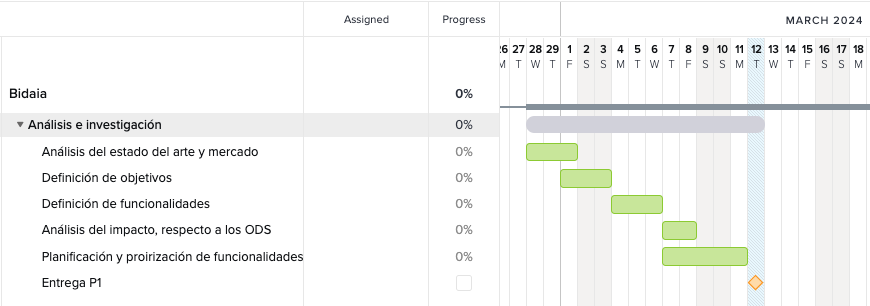
\includegraphics[width=0.95\textwidth]{Figures/Gantt/gantt-1.png}
\caption{Planificación del análisis}
\label{gantt-1}
\end{figure}

\begin{figure}[H]
\centering
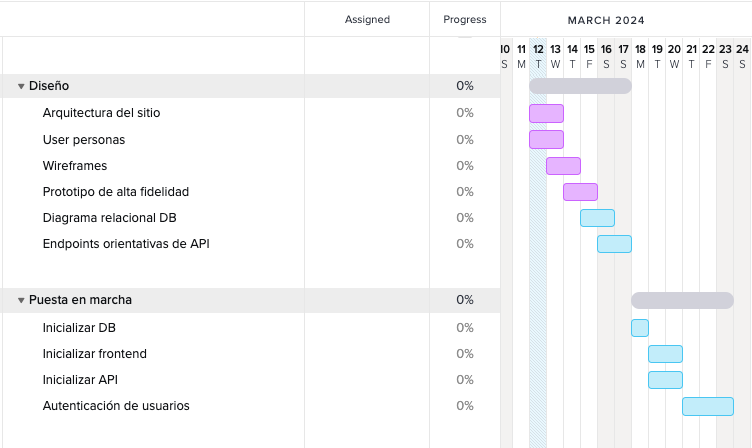
\includegraphics[width=0.95\textwidth]{Figures/Gantt/gantt-2.png}
\caption{Planificación del diseño y puesta en marcha}
\label{gantt-2}
\end{figure}

\begin{figure}[H]
\centering
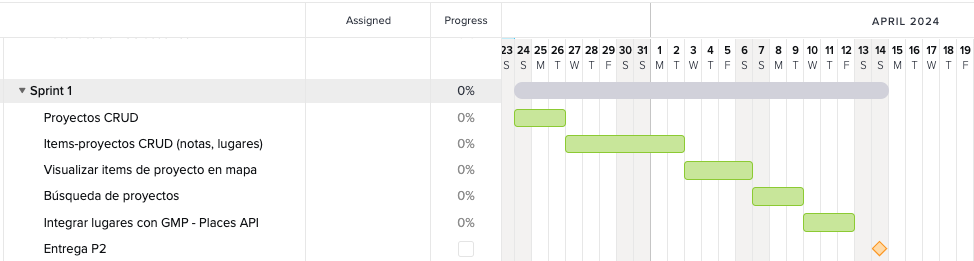
\includegraphics[width=0.95\textwidth]{Figures/Gantt/gantt-3.png}
\caption{Sprint 1}
\label{gantt-3}
\end{figure}

\begin{figure}[H]
\centering
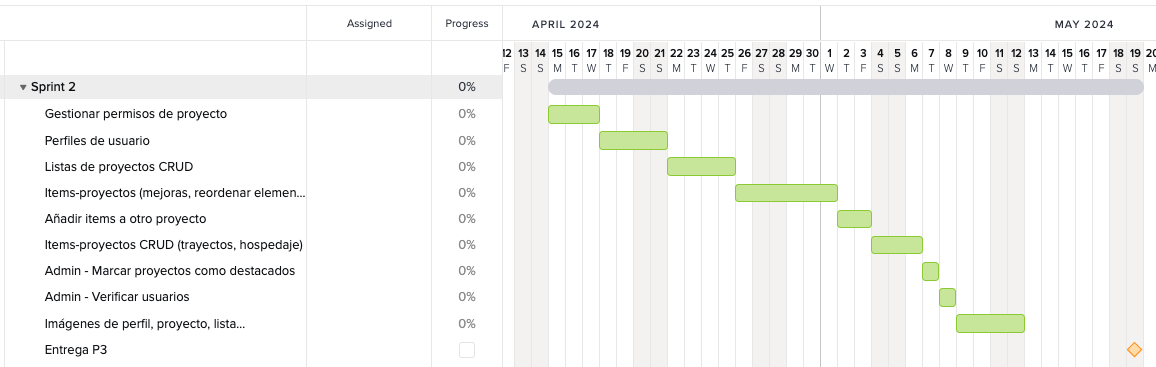
\includegraphics[width=0.95\textwidth]{Figures/Gantt/gantt-4.png}
\caption{Sprint 2}
\label{gantt-3}
\end{figure}


%%%%%%%%%%%%%%%%%%%%%%%%%%%%%%%%%%%%%%%%%%%%%%%%%%%%%%%%%%%%%%%%%%%%%%%%
\section{Breve sumario de productos obtenidos}
%%%%%%%%%%%%%%%%%%%%%%%%%%%%%%%%%%%%%%%%%%%%%%%%%%%%%%%%%%%%%%%%%%%%%%%%
Estos serían los activos obtenidos del desarrollo del trabajo:
\begin{itemize}
	\item Repositorio Git con el código fuente del frontend.
	\item Repositorio Git con el código fuente de la API.
	\item Memoria del proyecto.
	\item Documentación de la solución general.
	\item Documentación de la API.
	\item Guía para el despliegue, y los elementos que se utilicen (Dockerfile, Docker Compose...)
	\item Prototipos del diseño del frontend (archivos Figma).
\end{itemize}

%%%%%%%%%%%%%%%%%%%%%%%%%%%%%%%%%%%%%%%%%%%%%%%%%%%%%%%%%%%%%%%%%%%%%%%%
\section{Breve descripción de los otros capítulos de la memoria}
%%%%%%%%%%%%%%%%%%%%%%%%%%%%%%%%%%%%%%%%%%%%%%%%%%%%%%%%%%%%%%%%%%%%%%%%
En los siguientes capítulos se recogen las decisiones de diseño tomadas como el trascurso del desarrollo del proyecto:
\begin{itemize}
	\item Capítulo 2: Descripción de las decisiones de diseño tomadas y su justificación.
	\item Capítulo 3: Los resultados generados durante la duración del proyecto.
	\item Capítulo 4: Conclusiones obtenidas después de realizar el trabajo y las líneas de futuro.
	\item Capítulo 5,6,7:  Glosario, Siglas, Bibliografía y Anexos.
\end{itemize}
 


  %%%%%%%%%%%%%%%%%%%%%%%%%%%%%%%%%%%%%%%%%%%%%%%%%%%%%%%%%%%%%%%%%%%%%%%%
\chapter{Materiales y métodos}
%%%%%%%%%%%%%%%%%%%%%%%%%%%%%%%%%%%%%%%%%%%%%%%%%%%%%%%%%%%%%%%%%%%%%%%%


  %%%%%%%%%%%%%%%%%%%%%%%%%%%%%%%%%%%%%%%%%%%%%%%%%%%%%%%%%%%%%%%%%%%%%%%%
\chapter{Resultados}
%%%%%%%%%%%%%%%%%%%%%%%%%%%%%%%%%%%%%%%%%%%%%%%%%%%%%%%%%%%%%%%%%%%%%%%%

\iffalse
     Kapitulu honetan proiektuan garatutako lanak eta lortutako emaitzak azaltzen dira. Emaitzetara iristeko garatutako lanen definizio funtzionala eta azalpen teknikoak deskribatuz, eta arrazoibidean fokua jarriz.



%%%%%%%%%%%%%%%%%%%%%%%%%%%%%%%%%%%%%%%%%%%%%%%%%%%%%%%%%%%%%%%%%%%%%%%%
\section{Seccion...}
%%%%%%%%%%%%%%%%%%%%%%%%%%%%%%%%%%%%%%%%%%%%%%%%%%%%%%%%%%%%%%%%%%%%%%%%
Praktiken garapenean zehar burututako ekintzak ezagutu eta ulertzea ezinbestekoa da lortutako emaitzak lortzeko prozesua ezagutzeko. 

\subsection{Subseccion}\label{sec:bootcamp}
CYCn erabiltzen den \textit{stack} teknologikoa ezagutzeko, 3 hilabeteko \textit{bootcamp} motako formakuntza proposatu da
garapen inguruneak eta tresnak ezagutu, erabili eta barneratu ahal izateko. Formakuntza 6
kideko taldean burutu egin da, denok enpresan iritsi berriak. 3 zatitan banatu da formakuntza:
lehenik web teknologien oinarriak landu dira, ondoren Microsoft 365 ingurunean murgildu naiz
SharePoint eta Teams tresnetan fokua jarriz eta azkenik Microsoft Power Platformek
eskaintzen dituen Power Automate eta Power Apps \textit{no-code} edo \textit{low-code} tresnak landu dira soluzio
bizkorrak lortzeko. Prozesu honetan departamentu ezberdinetako kideak egon dira tutore
gisa. Atal bakoitza eduki teorikoekin hasi da, ondoren ariketa praktiko batean ikasitakoa
aplikatzeko eta azkenik beste kideekin eta tutorearekin berrikusi dira soluzio ezberdinak
aztertuz, tutoreen \textit{feedback}a lortzeko. 

\subsubsection{SubSubSeccion}
Enpresan lantzen diren proiektu asko \textit{web}an oinarritutako soluzioak izaten dira. Soluzio
hauek eraikitzeko \textit{Frontend}ean HTML, CSS eta JavaScript hirukote ezaguna eta \textit{Backend}ean
Microsoften .NET \textit{framework}a C\# lengoaiarekin batera erabiltzen dira.


\fi
  %%%%%%%%%%%%%%%%%%%%%%%%%%%%%%%%%%%%%%%%%%%%%%%%%%%%%%%%%%%%%%%%%%%%%%%%
\chapter{Conclusiones y líneas futuras}
%%%%%%%%%%%%%%%%%%%%%%%%%%%%%%%%%%%%%%%%%%%%%%%%%%%%%%%%%%%%%%%%%%%%%%%%

\iffalse
     Kapitulu honetan proiektuaren eta praktiken ondorioak jasotzen dira. Atal bakoitzean
     ikuspuntu ezberdinetatik azaltzen eta sakontzen da garatutako atazen inguruko gogoeta.



%%%%%%%%%%%%%%%%%%%%%%%%%%%%%%%%%%%%%%%%%%%%%%%%%%%%%%%%%%%%%%%%%%%%%%%%
\section{Ondorio ekonomikoak}
%%%%%%%%%%%%%%%%%%%%%%%%%%%%%%%%%%%%%%%%%%%%%%%%%%%%%%%%%%%%%%%%%%%%%%%%
\ref{sec:roi} atalean azaldu bezala, proiektuaren garapena ekonomikoki emankorra izan da. Nahiz eta formakuntzan eta lanerako materialean inbertsioa handia izan, bezero ezberdinetarako lanak burutu dira eta zerbitzu eta proiektu berriak eskaintzeko aukera berriak aztertu eta eraiki dira. Proiektuan zehar egindako lanen zati bat etorkizunean berrerabiltzeko eta probetxua ateratzeko aukera garbia dago.
%%%%%%%%%%%%%%%%%%%%%%%%%%%%%%%%%%%%%%%%%%%%%%%%%%%%%%%%%%%%%%%%%%%%%%%%
\section{Garapen Jasangarrirako Helburuekiko ondorioak}
%%%%%%%%%%%%%%%%%%%%%%%%%%%%%%%%%%%%%%%%%%%%%%%%%%%%%%%%%%%%%%%%%%%%%%%%
\acrfull{gjh} pertsonen, planetaren eta oparotasunaren aldeko ekintza-plan bat da, bake unibertsala eta justiziarako sarbidea indartzeko asmoa daukana \cite{gjh}. Nazio Batuen Erakundeak (\acrshort{nbe}) sortutako 17 helburu, 169 xede eta 231 adierazlez dago osatua eta Agenda 2030 planaren barruan aurkitzen da.

Proiektuan zehar garatutako emaitzek \acrshort{gjh}kiko duten inpaktua neurtzeko SDG Impact Assessment Tool\footnote{SDG Impact Assessment Tool \url{https://sdgimpactassessmenttool.org}}  tresna erabili da. Tresna honen bidez, helburu bakoitzerako inpaktua eta motibazioa deskribatu da. Informazio guzti honekin, \ref{gjh-guztiak} irudiko taula edo sailkapena lortu da. Helburu gehienek ez dute inpakturik jasaten garatutako proiektutik, baina badaude helburu batzuk zuzenean inpaktu positiboa dutenak, \ref{gjh-positiboak} irudian agertzen direnak alegia.

\begin{figure}[H]
\centering
\includegraphics[width=0.95\textwidth]{Figures/ondorioak/gjh-guztiak.png}
\caption{SDG Impact Assessment Tool tresnan lortutako emaitza}
\label{gjh-guztiak}
\end{figure}

\begin{figure}[H]
\centering
\includegraphics[width=0.8\textwidth]{Figures/ondorioak/gjh-positiboak.png}
\caption{Eragin zuzen positiboa lortu den helburuak}
\label{gjh-positiboak}
\end{figure}

Proiektuaren emaitzei erreparatuz (\ref{sec:emaitzak} atala), iradokizunen kudeaketari dagokion tresna da \acrshort{gjh}etan inpaktu gehien duena. Tresna honi esker lantokian egin daitezken hobekuntzak jaso, kudeatu eta exekutatzen dira. Hobekuntza hauek alor ezberdinetara egon daitezke zentratuta: segurtasun arriskuak minimizatzea, ekidin daitezken materialak kentzea, hondakin gutxiago sortzea, prozesu jasangarriagoak lortzeko urratsak hartzea... Tresna guztiz digitala denez, informazio sarrera eta jakinarazpen guztiak digitalki egiten dira eta paperaren erabilera minimora jaitsi da. Soluzioak 3., 12. eta 15. helburuetan du inpaktu zuzena: osasuna eta ongizatea, ekoizpen eta kontsumo arduratsuak, lehorreko ekosistemetako bizitza. 

Proiektu osoak langileentzako plataforma digital bat izan du ardatz eta industria sektoreko erakunde baten barruan egin da. Erakundearentzat aldaketa handia izan, kolaboraziorako aukerak maximizatuz eta komunikazioa erraztuz. Lanerako modua eraldatzeagatik 9. helburuan jaso da inpaktu positibo zuzena, industria, berrikuntza eta azpiegiturarena. 



SDG Impact Assessment Tool tresnaren bidez lortutako emaitza osoa eta egindako iruzkinak \ref{app:gjh} eranskinean aurkitzen dira. 

\fi
  
  
%PARAGRAPH STYLE
\setlength\parskip{1em plus 0.1em minus 0.2em}
\setlength\parindent{0pt}

% This ensures that the subsequent sections are being included as root
% items in the bookmark structure of your PDF reader.
\bookmarksetup{startatroot}
\backmatter
  \begingroup
    \let\clearpage\relax
    \glsaddall
    \renewcommand{\glsnamefont}[1]{\textbf{#1}}
    \printglossary[type=\acronymtype]
    \newpage
    \printglossary
  \endgroup
  
  \printindex
  \printbibliography
  
  %%%%%%%%%%%%%%%%%%%%%%%%%%%%%%%%%%%%%%%%%%%%%%%%%%%%%%%%%%%%%%%%%%%%%%%%
%% Eranskinak
%%%%%%%%%%%%%%%%%%%%%%%%%%%%%%%%%%%%%%%%%%%%%%%%%%%%%%%%%%%%%%%%%%%%%%%%

\pagestyle{appendix}
\vspace*{\fill}
{\Huge\textsc{Anexos}}
\addcontentsline{toc}{chapter}{Anexos}
\vspace*{\fill}

\appendix
\renewcommand{\thesection}{\Alph{section}}

%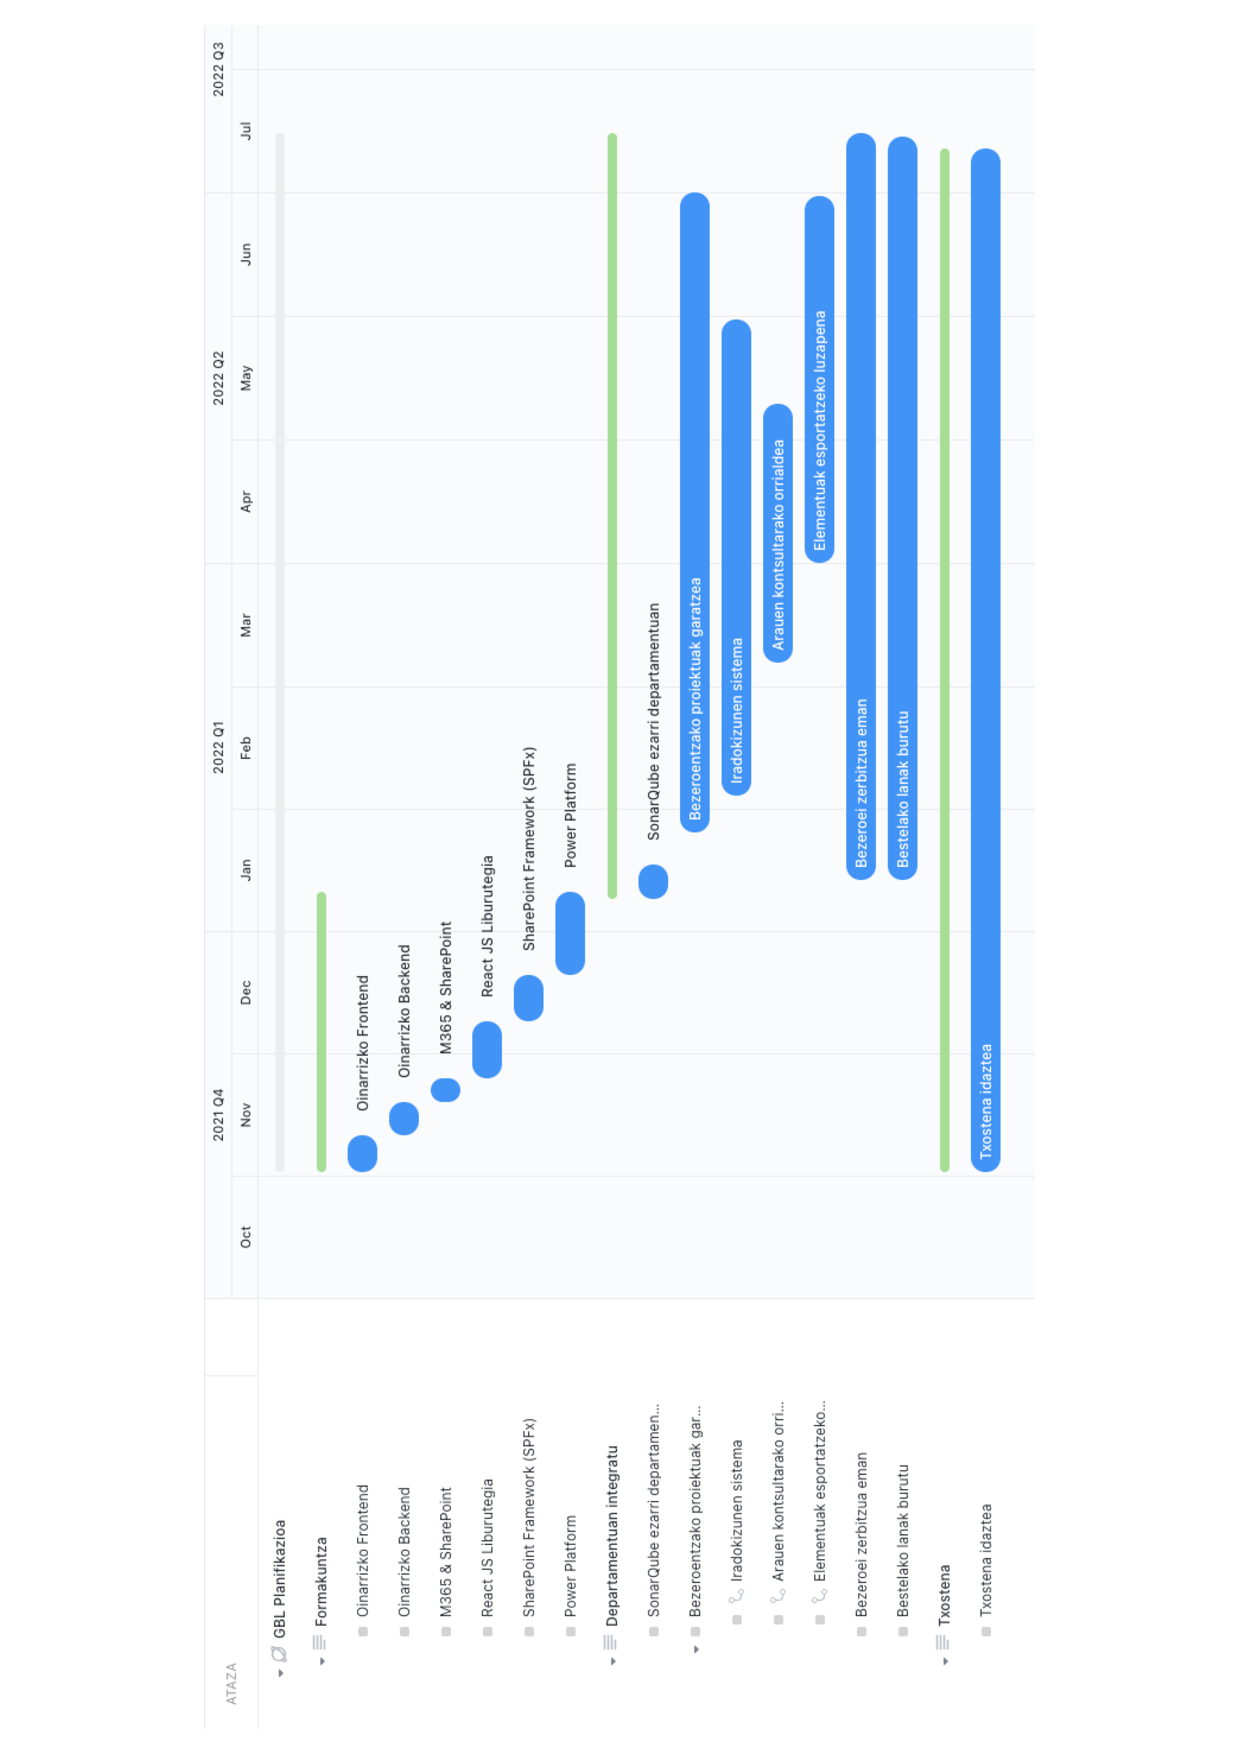
\includepdf[scale=0.75, pages=1, angle=180, pagecommand=\section{Proiektuaren planifikazioaren Gantt diagrama}\label{app:gantt}]{Assets/gantt-final.pdf}

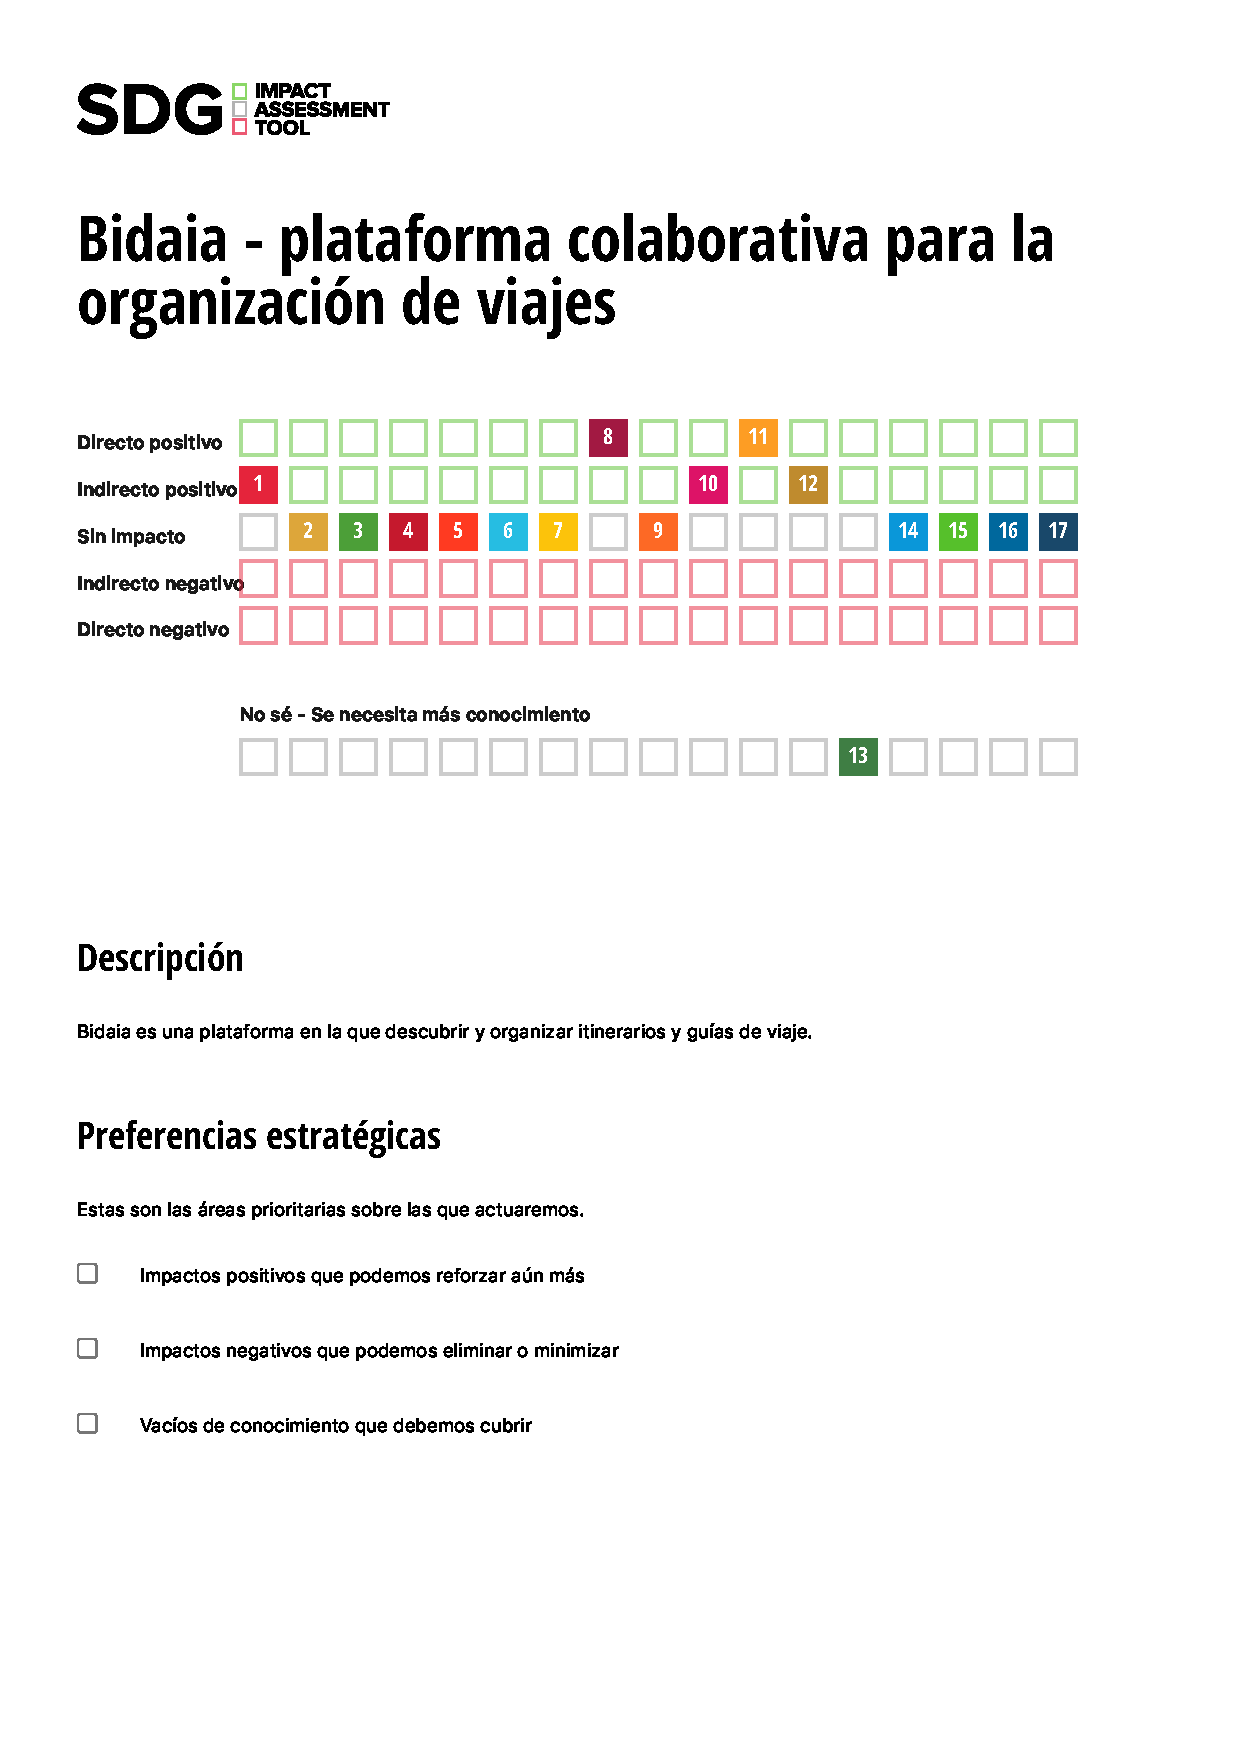
\includepdf[scale=0.75, pages=1,pagecommand=\section{El impacto del proyecto respecto a los ODS}\label{app:gjh}]{Assets/bidaia-sdg.pdf}
\includepdf[scale=0.80, pages=2-last, pagecommand=\thispagestyle{eranskinak}]{Assets/bidaia-sdg.pdf}

\pagestyle{plain}





\end{document}
